% =================================================================================================
% File:			registrazione_e_autenticazione.tex
% Description:	Definisce la sezione relativa ad un capitolo del documento
% Created:		2015-04-21
% Author:		Santacatterina Luca
% Email:		santacatterina.luca@mashup-unipd.it
% =================================================================================================
% Modification History:
% Version		Modifier Date		Change											Author
% 0.0.1 		2015-05-24 			inizio stesura sezione capitolo					Santacatterina Luca
% =================================================================================================
%

% CONTENUTO DEL CAPITOLO
\section{Registrazione e autenticazione} % (fold)
\label{sec:registrazione e autenticazione}
	In questa sezione saranno descritte le funzionalità di registrazione e autenticazione\gloss{} fornite all'utente nella fase iniziale.


	\subsection{Registrazione} % (fold)
	\label{sec:registrazione}
		Per ogni sezione vengono riportati screenshot\gloss{} illustrativi per agevolare la comprensione del funzionamento.


		\subsubsection{Utente non autenticato} % (fold)
		\label{sec:utente_non_autenticati}
			Prima di iniziare l'utilizzo del software \projectName{} è richiesta la registrazione.\newline
			Per poter proseguire è necessario cliccare su link \textbf{Register} presente nella prima pagina del sito (Figura: \ref{fig:registrazione_utente_accesso}).
			\begin{figure}[H]
				\centering
				\centerline{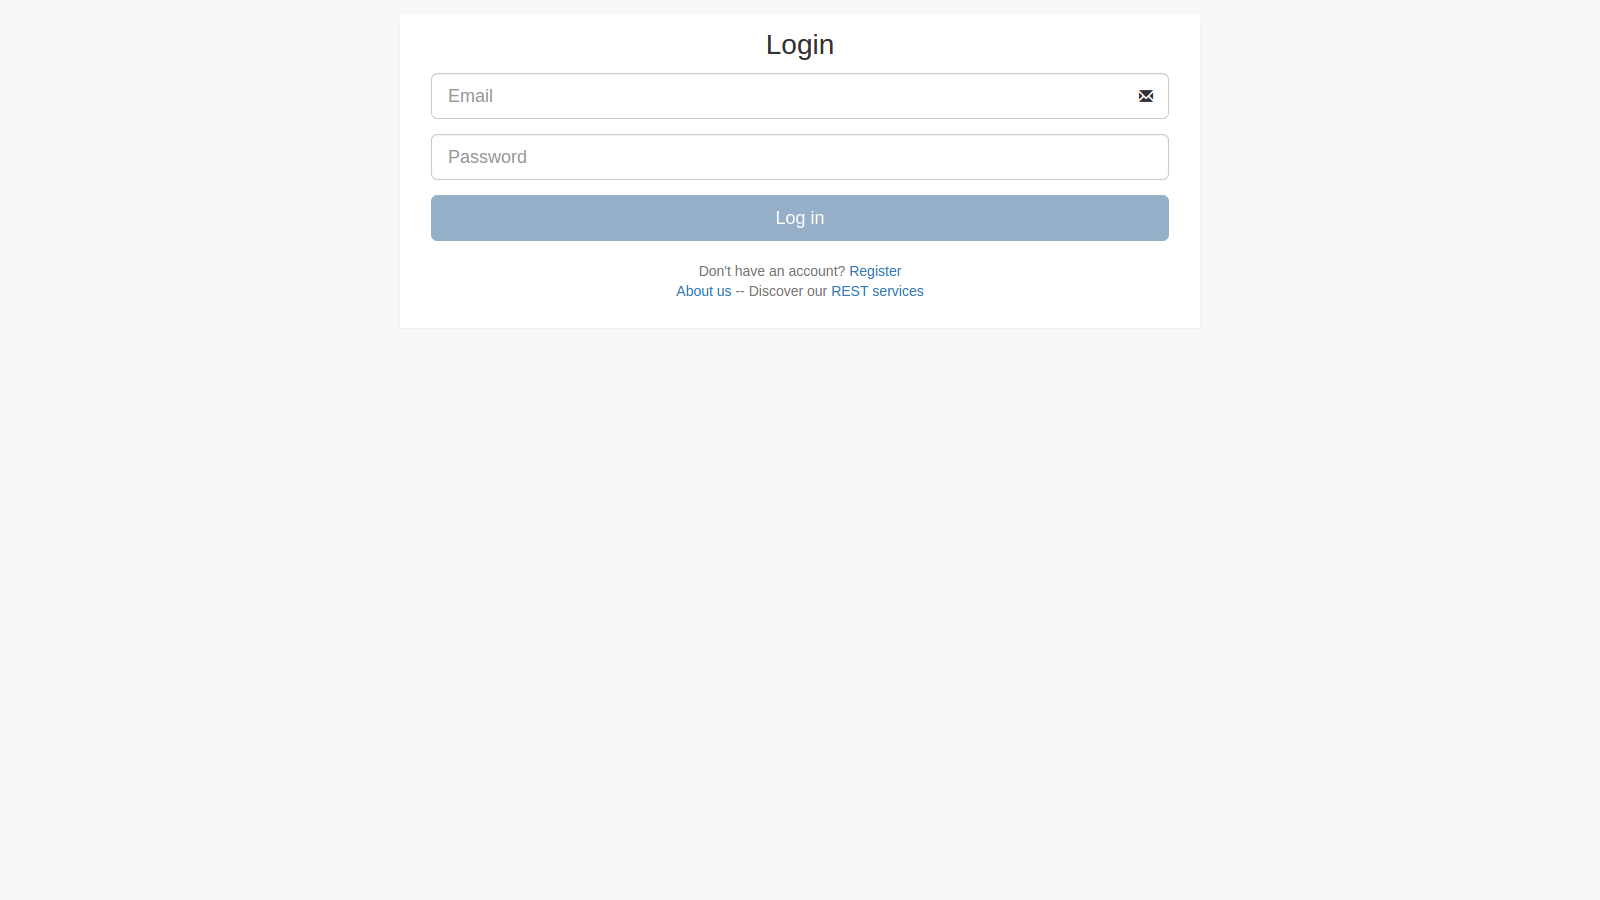
\includegraphics[width=14cm]{images/registrazione_utente_accesso.png}}
				\caption{Accesso registrazione all'applicazione}
				\label{fig:registrazione_utente_accesso}
			\end{figure}
		% section Utente non autenticato (end)

		\pagebreak
		\subsubsection{Compilazione dati utente} % (fold)
		\label{sec:compilazioni_dati_utente}
			Per poter proseguire è necessaria l'inserimento di tutti i dati obbligatori (Figura: \ref{fig:pagina_di_registrazione}).
			\begin{figure}[H]
				\centering
				\centerline{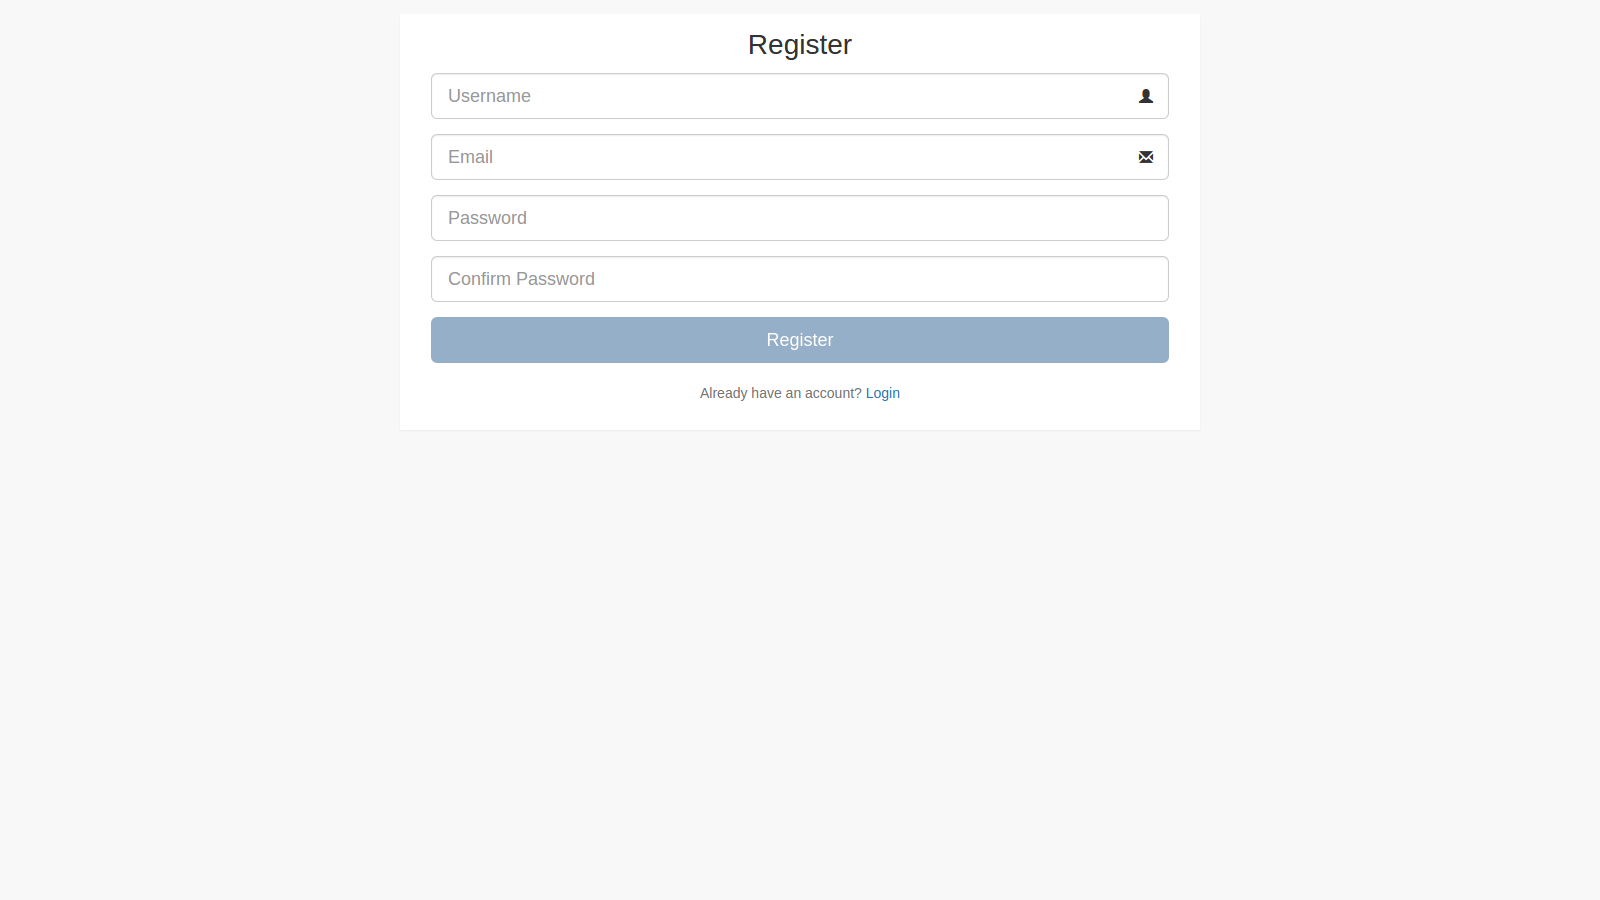
\includegraphics[width=14cm]{images/registrazione_utente.png}}
				\caption{Pagina di registrazione}
				\label{fig:pagina_di_registrazione}
			\end{figure}
			È presente un \textbf{form}\gloss{} da completare con i seguenti dati:
			\begin{itemize}
				\item \textbf{Username}: inserire un username per l'accesso non già presente nell'applicazione;
				\item \textbf{Email}:inserire un indirizzo email valido;
				\item \textbf{Password}: inserire password di registrazione;
				\item \textbf{Confirm Password}: inserire nuovamente la password del punto precedente.
			\end{itemize}
			Se la compilazione dei campi è avvenuta correttamente è possibile vedere l'abilitazione e quindi il cambiamento di colore del pulsante \textbf{Register}.\\
			Dopo aver premuto il pulsante si caricherà automaticamente la pagina per l'autenticazione\gloss{} (Figura: \ref{fig:registrazione_utente_accesso}).
		% section Compilazione dati utente (end)

		\pagebreak
		\subsubsection{Autenticazione utente} % (fold)
		\label{sec:autenticazione_utente}
			Per effettuare l'autenticazione\gloss{} all'applicazione si devono inserire:
			\begin{itemize}
				\item Email;
				\item Password.
			\end{itemize}
			\begin{figure}[H]
				\centering
				\centerline{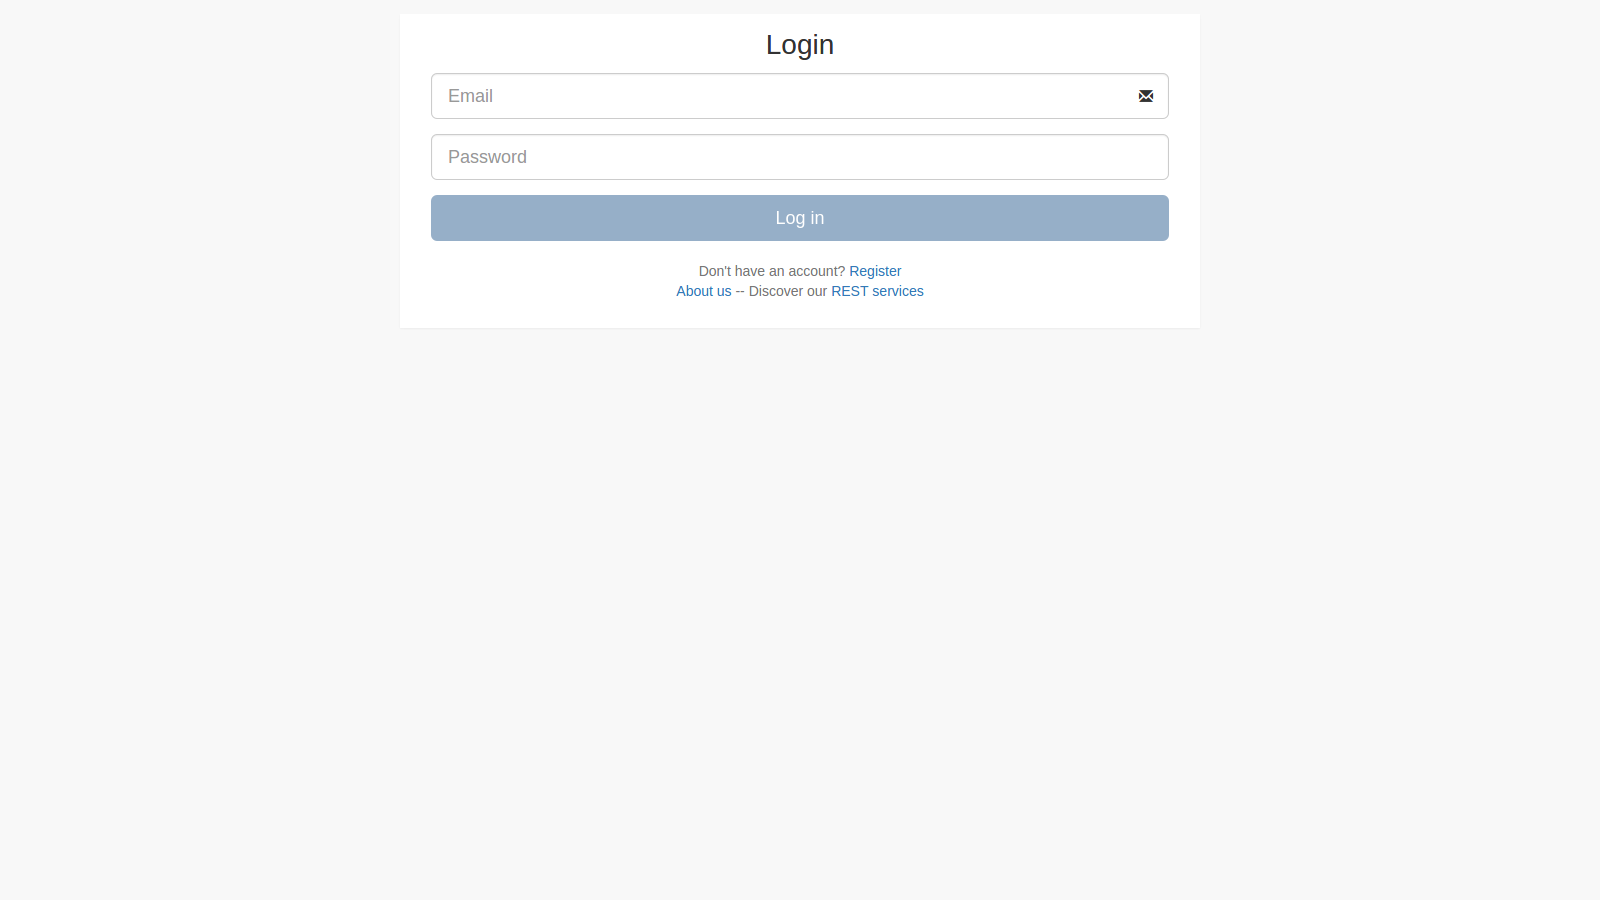
\includegraphics[width=14cm]{images/autenticazione_utente.png}}
				\caption{Autenticazione utente}
				\label{fig:registrazione_utente_accesso}
			\end{figure}
			Dopo aver inserito i dati di autenticazione (Figura \ref{fig:registrazione_utente_accesso}) sarà possibile premere il pulsante \textbf{Login}\gloss{} e quindi si verrà collegati alla dashboard\gloss{} dell'applicazione (Figura: \ref{fig:dashboard})
			\begin{figure}[H]
				\centering
				\centerline{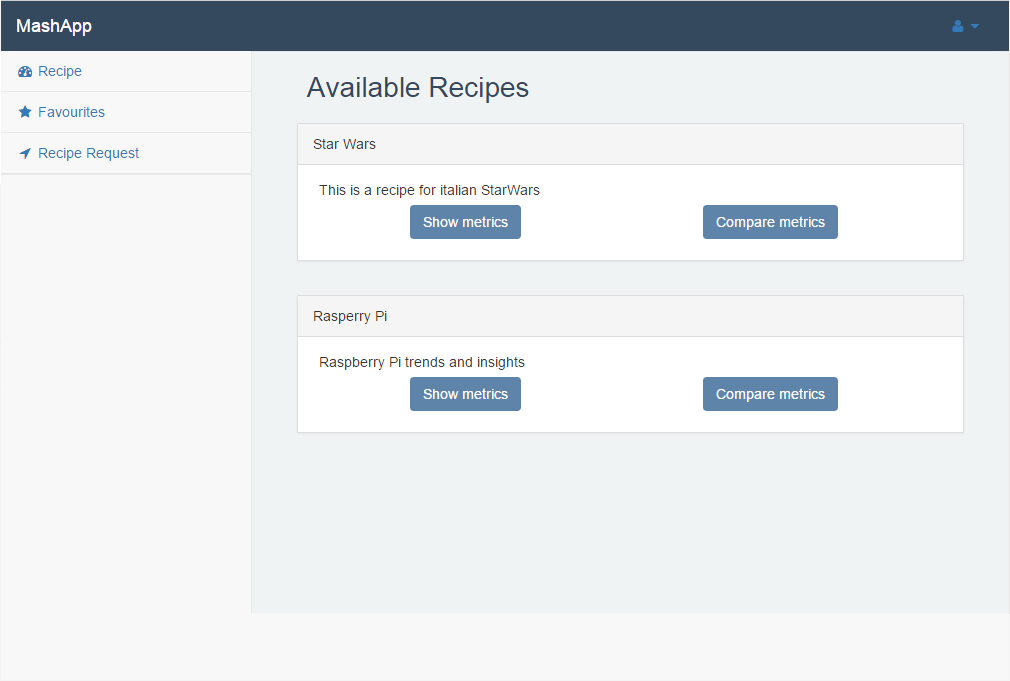
\includegraphics[width=19cm]{images/dashboard.png}}
				\caption{Dashboard applicazione}
				\label{fig:dashboard}
			\end{figure}
		% section Autenticazione utente (end)


	% section Registrazione (end)

% section Registrazione e autenticazione (end)